\documentclass[10pt]{article}
\usepackage[a4paper,margin=14mm]{geometry}
\usepackage[T1]{fontenc}
\usepackage[utf8]{inputenc}
\usepackage{lmodern}
\usepackage{tikz}
\usetikzlibrary{arrows.meta,positioning,calc}
\usepackage{tabularx,array,booktabs}
\pagestyle{empty}
\setlength{\parindent}{0pt}

% Review boxes are the only coloured elements.
% Set \reviewcolourfalse for a completely black-and-white version.
\newif\ifreviewcolour
\reviewcolourtrue
\ifreviewcolour
  \definecolor{reviewfill}{HTML}{E8F0EB}
\else
  \definecolor{reviewfill}{gray}{0.92}
\fi

\begin{document}
\begin{center}
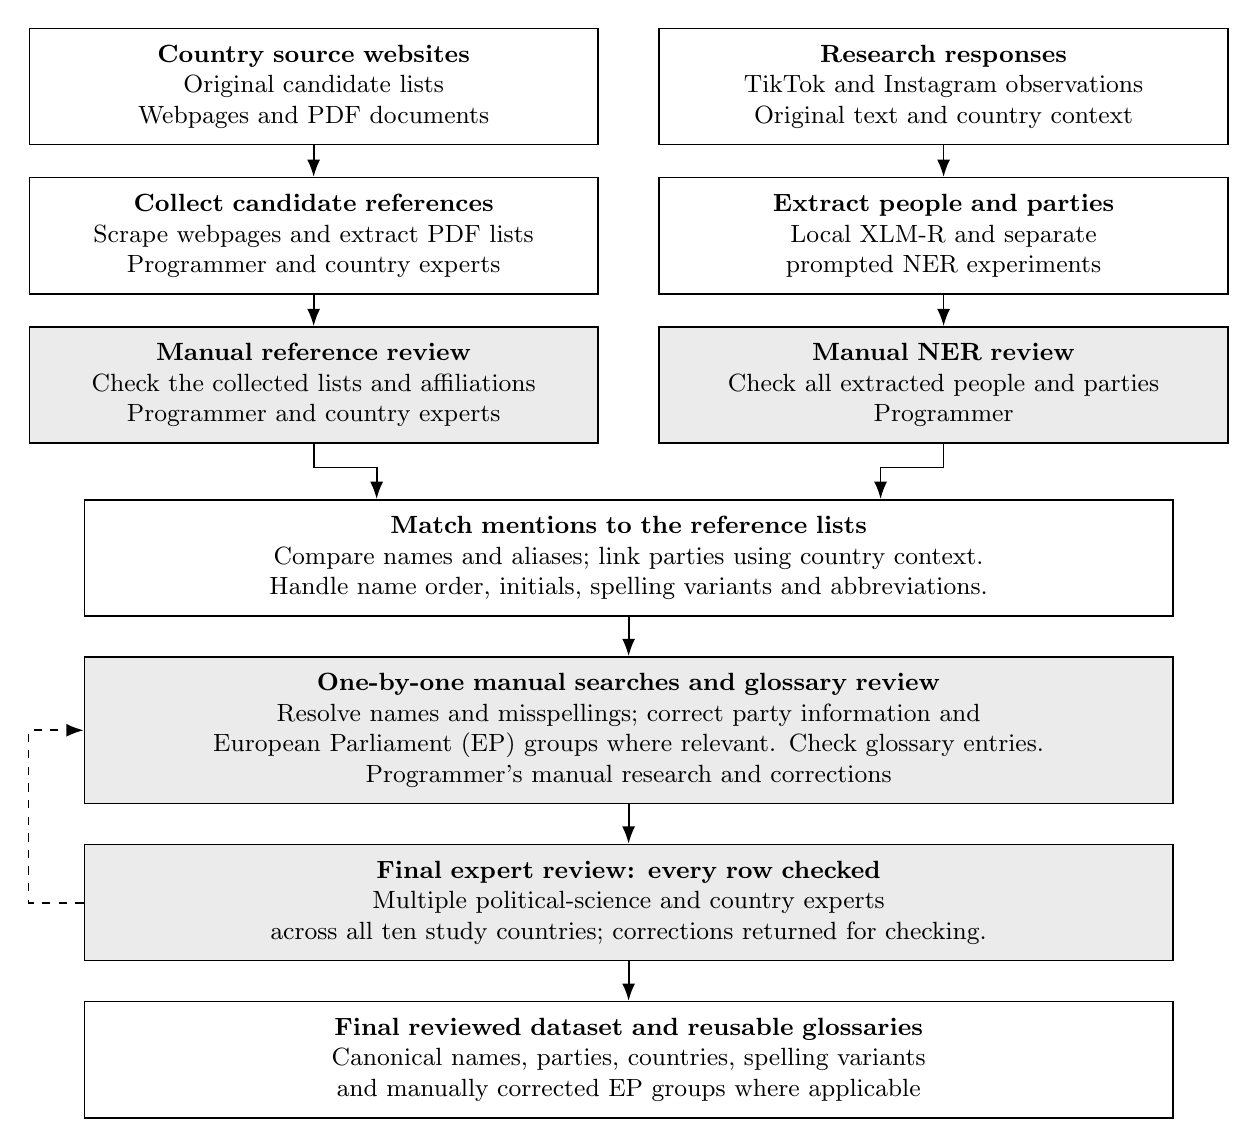
\begin{tikzpicture}[
  box/.style={
    draw=black,line width=0.55pt,fill=white,
    text width=6.8cm,align=center,inner sep=6pt,
    font=\fontsize{9}{11}\selectfont
  },
  review/.style={box,fill=reviewfill},
  wide/.style={text width=13.4cm},
  arrow/.style={-{Latex[length=2.2mm]},draw=black,line width=0.65pt}
]

\node[box] (sources) at (-4,0) {
  \textbf{Country source websites}\\
  Original candidate lists\\
  Webpages and PDF documents
};
\node[box] (responses) at (4,0) {
  \textbf{Research responses}\\
  TikTok and Instagram observations\\
  Original text and country context
};

\node[box,below=4mm of sources] (scrape) {
  \textbf{Collect candidate references}\\
  Scrape webpages and extract PDF lists\\
  Programmer and country experts
};
\node[box,below=4mm of responses] (ner) {
  \textbf{Extract people and parties}\\
  Local XLM-R and separate\\
  prompted NER experiments
};

\node[review,below=4mm of scrape] (refcheck) {
  \textbf{Manual reference review}\\
  Check the collected lists and affiliations\\
  Programmer and country experts
};
\node[review,below=4mm of ner] (nercheck) {
  \textbf{Manual NER review}\\
  Check all extracted people and parties\\
  Programmer
};

\coordinate (join) at
  ($(refcheck.south)!0.5!(nercheck.south)$);
\node[box,wide,below=7mm of join] (link) {
  \textbf{Match mentions to the reference lists}\\
  Compare names and aliases; link parties using country context.\\
  Handle name order, initials, spelling variants and abbreviations.
};
\node[review,wide,below=5mm of link] (curate) {
  \textbf{One-by-one manual searches and glossary review}\\
  Resolve names and misspellings; correct party information and\\
  European Parliament (EP) groups where relevant. Check glossary entries.\\
  Programmer's manual research and corrections
};
\node[review,wide,below=5mm of curate] (finalcheck) {
  \textbf{Final expert review: every row checked}\\
  Multiple political-science and country experts\\
  across all ten study countries; corrections returned for checking.
};
\node[box,wide,below=5mm of finalcheck] (output) {
  \textbf{Final reviewed dataset and reusable glossaries}\\
  Canonical names, parties, countries, spelling variants\\
  and manually corrected EP groups where applicable
};

\draw[arrow] (sources) -- (scrape);
\draw[arrow] (scrape) -- (refcheck);
\draw[arrow] (responses) -- (ner);
\draw[arrow] (ner) -- (nercheck);
\draw[arrow] (refcheck.south) -- ++(0,-3mm)
  -| ([xshift=-3.2cm]link.north);
\draw[arrow] (nercheck.south) -- ++(0,-3mm)
  -| ([xshift=3.2cm]link.north);
\draw[arrow] (link) -- (curate);
\draw[arrow] (curate) -- (finalcheck);
\draw[arrow] (finalcheck) -- (output);
\draw[arrow,dashed] (finalcheck.west) -- ++(-7mm,0)
  |- (curate.west);

\end{tikzpicture}
\end{center}

\vspace{3mm}
\renewcommand{\arraystretch}{1.2}
\small
\begin{tabularx}{\linewidth}{@{}>{\bfseries}p{3.9cm} X@{}}
\toprule
What improved & \textbf{How the work handles it} \\
\midrule
Different name orders &
Token-set matching and saved aliases:
Magyar P\'{e}ter / P\'{e}ter Magyar. \\
Misspellings and short names &
Fuzzy matching plus manually recorded variants. \\
Party affiliation &
Person-to-party references, local party names and abbreviations. \\
Country ambiguity &
Country preference in the party pass; separate actor-country lookup. \\
Reusable manual work &
Ten country glossaries: 2,006 rows and 3,401 variant items. \\
\bottomrule
\end{tabularx}
\end{document}
